% Lightning talk, DevFest Milano 2026 (Saturday 10 October 2026, 11:30)
% Colours follow the business card - navy, blue, black and white
% Compile with  tectonic gdg_lightning.tex
\documentclass[aspectratio=169,11pt]{beamer}
\usepackage{graphicx}
\usepackage{booktabs}
\usepackage{ragged2e}
\usepackage{qrcode}
\usefonttheme{professionalfonts}

\definecolor{malam}{RGB}{11,27,48}       % navy background
\definecolor{birumuda}{RGB}{122,162,255} % light blue on navy
\definecolor{biru}{RGB}{40,84,200}       % blue accent on white
\definecolor{tinta}{RGB}{20,20,20}       % black text

\setbeamercolor{normal text}{fg=tinta,bg=white}
\setbeamercolor{structure}{fg=biru}
\setbeamercolor{frametitle}{fg=malam,bg=white}
\setbeamerfont{frametitle}{series=\bfseries,size=\Large}
\setbeamertemplate{navigation symbols}{}
\setbeamertemplate{itemize item}{\color{biru}\rule[0.25ex]{0.45em}{0.45em}}
\setbeamersize{text margin left=0.9cm,text margin right=0.9cm}
\setbeamertemplate{frametitle}{\vspace{0.45cm}\insertframetitle\par\vspace{0.1cm}{\color{biru}\rule{1.6cm}{1.5pt}}}
\setbeamertemplate{footline}{\hspace{0.9cm}{\tiny\color{tinta!45}Jessica Syafaq Muthmaina \textperiodcentered{} DevFest Milano 2026}\hfill{\tiny\color{tinta!45}\insertframenumber}\hspace*{0.9cm}\par\vspace{0.3cm}}

% source line under a figure or a quotation
\newcommand{\src}[1]{{\par\vspace{0.35em}\scriptsize\color{tinta!60}Source - #1\par}}
\newcommand{\kunci}[1]{{\bfseries\color{biru}#1}}

\begin{document}

% 1 title ----------------------------------------------------
{\setbeamercolor{background canvas}{bg=malam}\setbeamertemplate{footline}{}
\begin{frame}[plain]
  \vspace{1.0cm}
  {\raggedright\color{birumuda}\bfseries\fontsize{28}{36}\selectfont AI Wrote It, You Pushed It,\\ Who Checks It?\par}
  \vspace{0.6em}{\color{birumuda}\rule{2.6cm}{1.2pt}}\par\vspace{0.9em}
  {\raggedright\color{white}\large What astrophysics learned from decades of trusting code\par}
  \vspace{1.1cm}
  {\raggedright\color{white}Jessica Syafaq Muthmaina\par}
  \vspace{0.2em}
  {\raggedright\color{white!70!malam}\small MSc Astrophysics and Cosmology, University of Padua\par}
  \vspace{0.2em}
  {\raggedright\ttfamily\scriptsize\color{white!60!malam}@your.astrophysicist \textperiodcentered{} DevFest Milano, 10 October 2026\par}
  \vfill
\end{frame}}

% 2 about me -------------------------------------------------
\begin{frame}{About me}
  \begin{columns}[c,onlytextwidth]
    \begin{column}{0.64\textwidth}
      {\raggedright\color{malam}\bfseries Jessica Syafaq Muthmaina\par}
      {\raggedright\small\color{biru}a BRAT astrophysicist\par}
      \vspace{0.35em}
      \small
      \begin{itemize}\setlength{\itemsep}{0.45em}
        \item MSc Astrophysics and Cosmology, University of Padua, observational and computational track (2025 to now)
        \item BSc Physics, Universitas Gadjah Mada, Indonesia, theoretical and computational track (2019 to 2023)
        \item Research intern at BRIN, Indonesia's national research agency, working on 33 years of radio telescope data
        \item Data science intern, then data analyst in Indonesia
      \end{itemize}
    \end{column}
    \begin{column}{0.30\textwidth}
      \centering
      {\color{malam}\qrcode[height=3.3cm]{https://www.yourastro.space/}}\par
      \vspace{0.5em}
      {\ttfamily\small\color{biru}yourastro.space\par}
    \end{column}
  \end{columns}
\end{frame}

% premise (added 8 October 2026, night) ----------------------
\begin{frame}{Where I start}
  \vspace{0.5cm}
  {\raggedright\fontsize{19}{26}\selectfont\color{malam}
  More and more projects are made with AI\\[0.25em]
  and published straight to \kunci{GitHub} or \kunci{arXiv}.\\[0.25em]
  Publishing is easy. \kunci{Checking is not.}\par}
  \vspace{0.8cm}
  {\raggedright The distance between the two worries me. One night this month showed how big it is.\par}
\end{frame}

% 2 the drop -------------------------------------------------
\begin{frame}{One upload, 722 papers}
  \begin{columns}[c,onlytextwidth]
    \begin{column}{0.50\textwidth}
      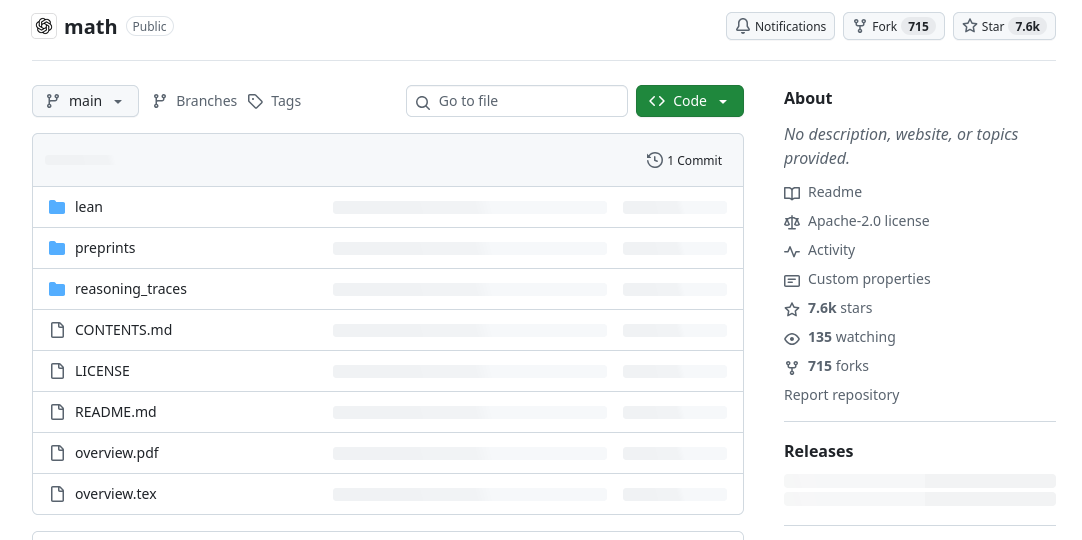
\includegraphics[width=\linewidth]{figs/shot_repo_top.png}
      \src{OpenAI (2026a), screenshot taken 7 October 2026}
    \end{column}
    \begin{column}{0.46\textwidth}
      \begin{itemize}\setlength{\itemsep}{0.7em}
        \item On 6 October 2026, OpenAI put \kunci{722} math papers online in one night.
        \item No person wrote them. \kunci{An AI program did.}
        \item It was given \kunci{4,000} math problems that nobody had solved yet.
      \end{itemize}
    \end{column}
  \end{columns}
\end{frame}

% 3 the person -----------------------------------------------
\begin{frame}{Twenty-four years, one night}
  \centering
  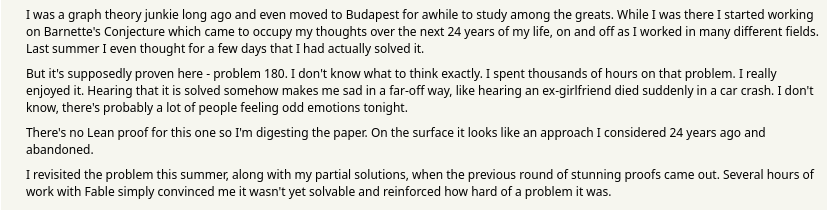
\includegraphics[width=0.92\linewidth]{figs/shot_hn_comment.png}
  \src{comment on Hacker News (2026), posted 7 October 2026}
  \vspace{0.8em}
  \raggedright
  A stranger online reads that a problem they worked on for 24 years is now ``supposedly proven''. Later they add that they never lost a single hour on it. ``Those were all hours that I gained.''
\end{frame}

% 4 my lab ---------------------------------------------------
\begin{frame}{My laboratory is code}
  \begin{columns}[c,onlytextwidth]
    \begin{column}{0.48\textwidth}
      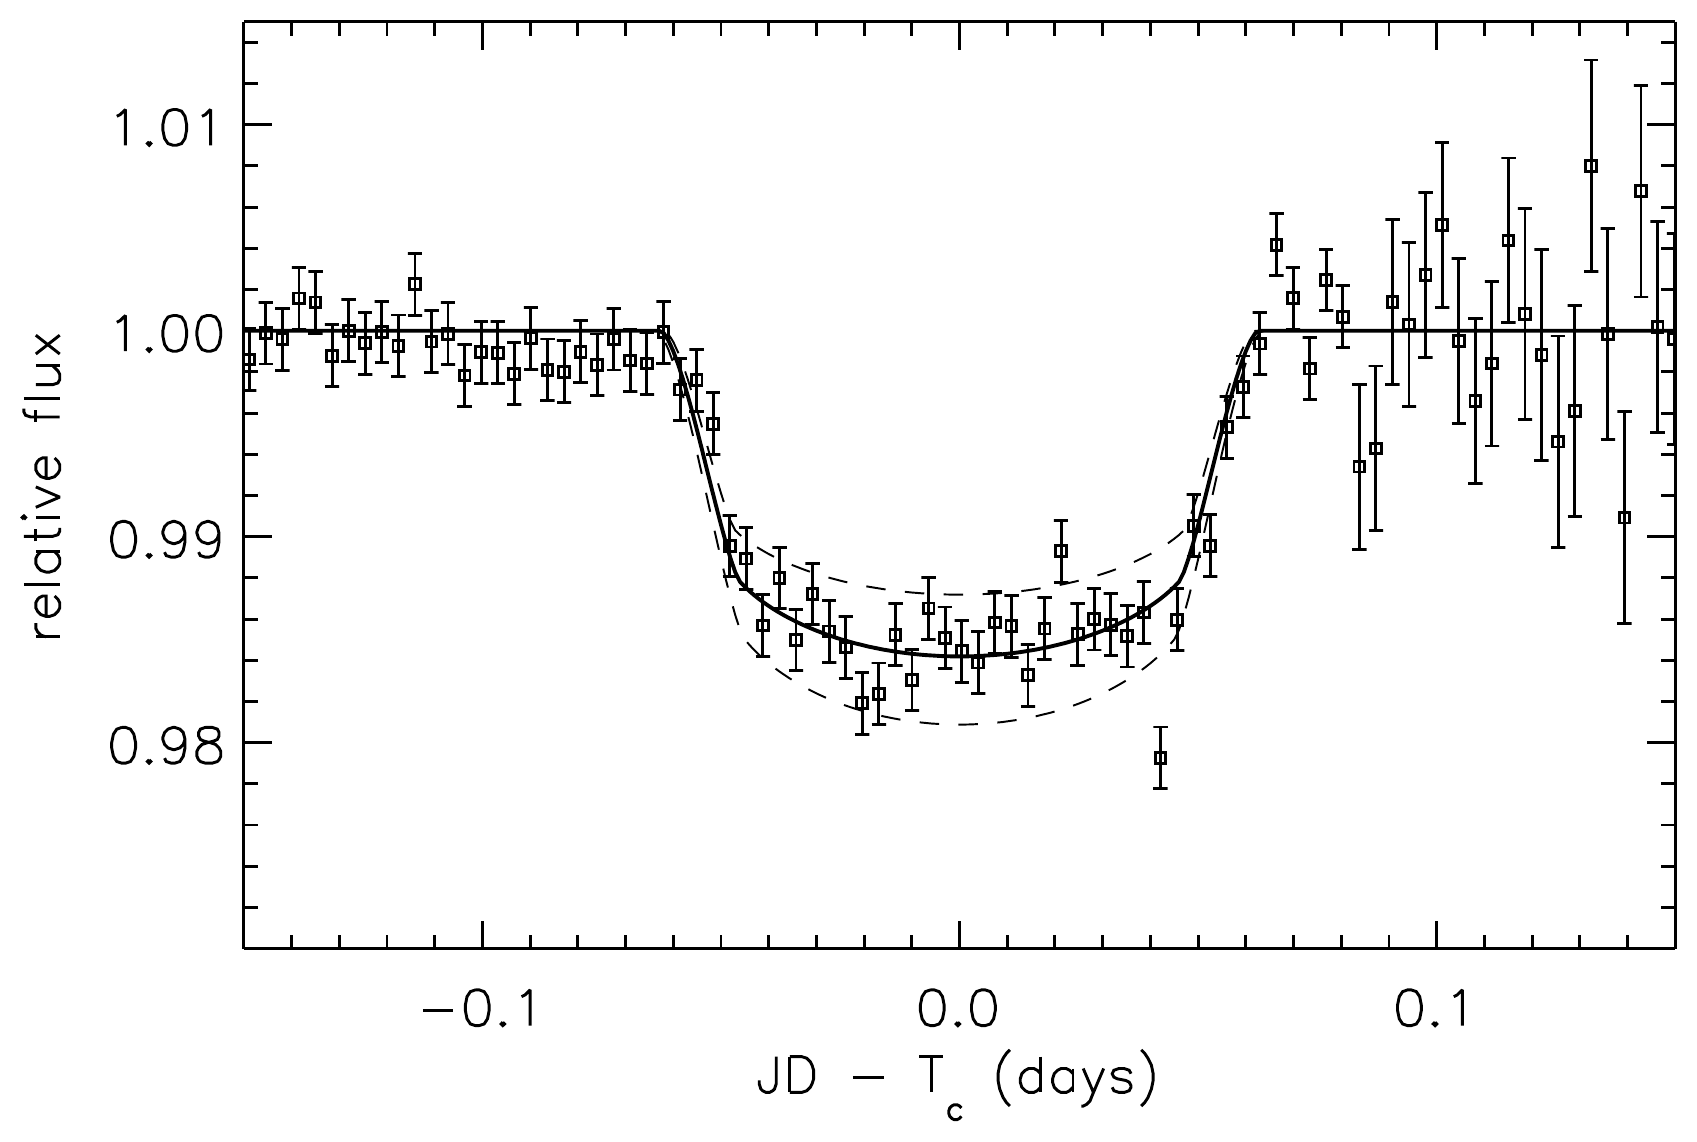
\includegraphics[width=\linewidth]{figs/charbonneau2000_fig2.png}
      \src{Charbonneau et al. (2000), Figure 2}
    \end{column}
    \begin{column}{0.48\textwidth}
      \begin{itemize}\setlength{\itemsep}{0.5em}
        \item I cannot bring a star into a lab. I can only watch it from far away.
        \item When a planet passes in front of its star, it blocks a little of the light.
        \item Here the star lost \kunci{less than 2 percent} of its light. That small dip is the planet.
        \item It was the first planet caught this way, in 1999. Nobody saw it. A computer calculation says it is there.
      \end{itemize}
    \end{column}
  \end{columns}
\end{frame}

% 5 machines already in the room -----------------------------
\begin{frame}{The machines were already in the room}
  \begin{columns}[c,onlytextwidth]
    \begin{column}{0.56\textwidth}
      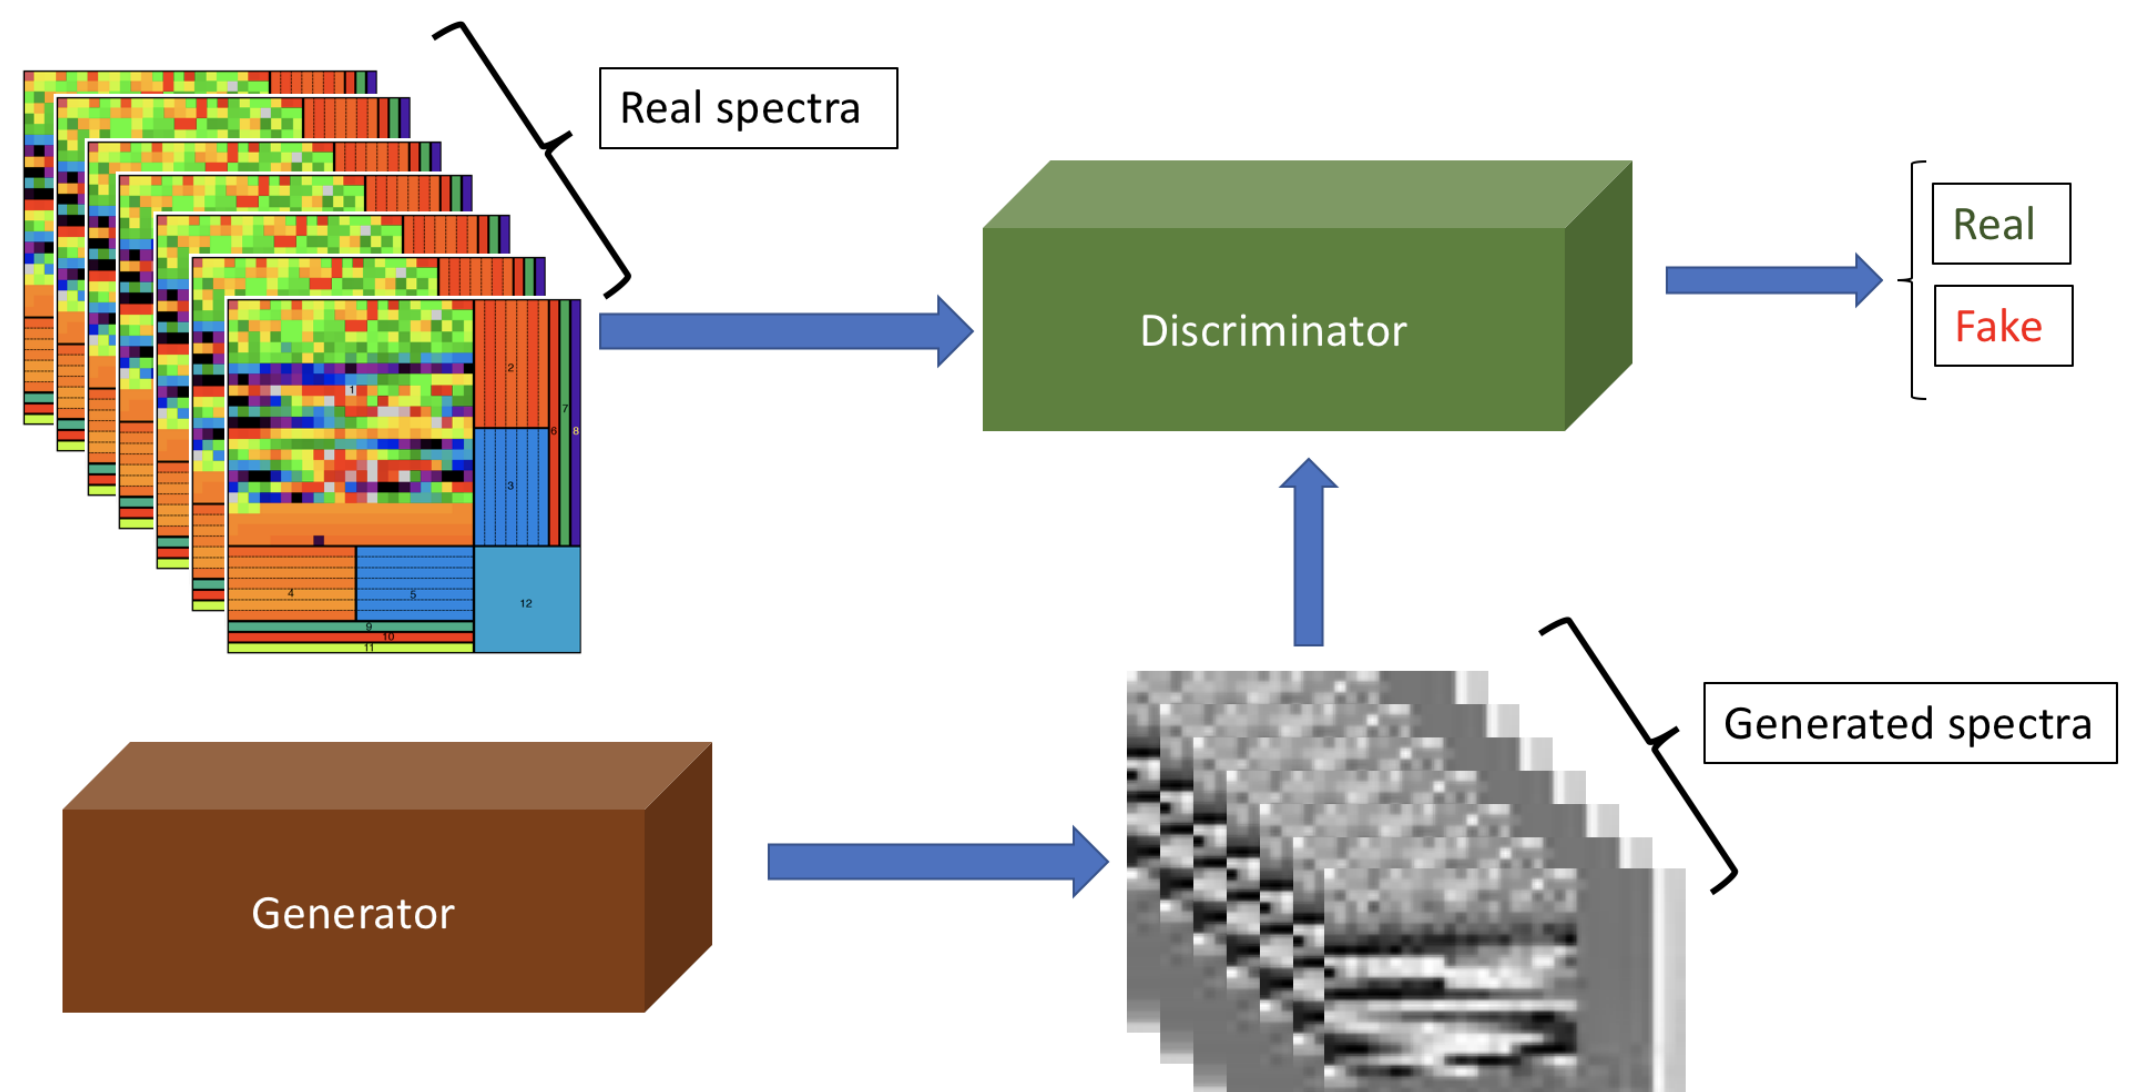
\includegraphics[width=\linewidth]{figs/zingales2018_fig1.png}
      \src{Zingales and Waldmann (2018), Figure 1}
    \end{column}
    \begin{column}{0.40\textwidth}
      \begin{itemize}\setlength{\itemsep}{0.7em}
        \item In 2018 an AI program learned to guess what the air of a distant planet is made of.
        \item One of its authors now teaches my course.
        \item My field did not fall apart. The paper and the code are public, so anyone can run it again and check.
      \end{itemize}
    \end{column}
  \end{columns}
\end{frame}

% the flood (added 8 October 2026) ---------------------------
\begin{frame}{Astronomy already has a flood of data}
  \vspace{0.1cm}
  {\raggedright\fontsize{17}{23}\selectfont\color{malam}
  The Gaia telescope has listed \kunci{1.8 billion} stars.\\[0.25em]
  The Euclid telescope is mapping \kunci{a third of the sky}.\\[0.25em]
  No person can look at them all, one by one.\par}
  \vspace{0.45cm}
  {\raggedright So a computer looks first.\\ My job is to know the physics well enough to say \kunci{this one is wrong}.\par}
  \vspace{0.3cm}
  {\raggedright That is why I still study.\par}
  \vspace{0.25cm}
  \src{Gaia Collaboration (2023) and Euclid Collaboration (2025)}
\end{frame}

% the UV map (added 9 October 2026) --------------------------
\begin{frame}{Made with AI, checked by a person}
  \begin{columns}[c,onlytextwidth]
    \begin{column}{0.46\textwidth}
      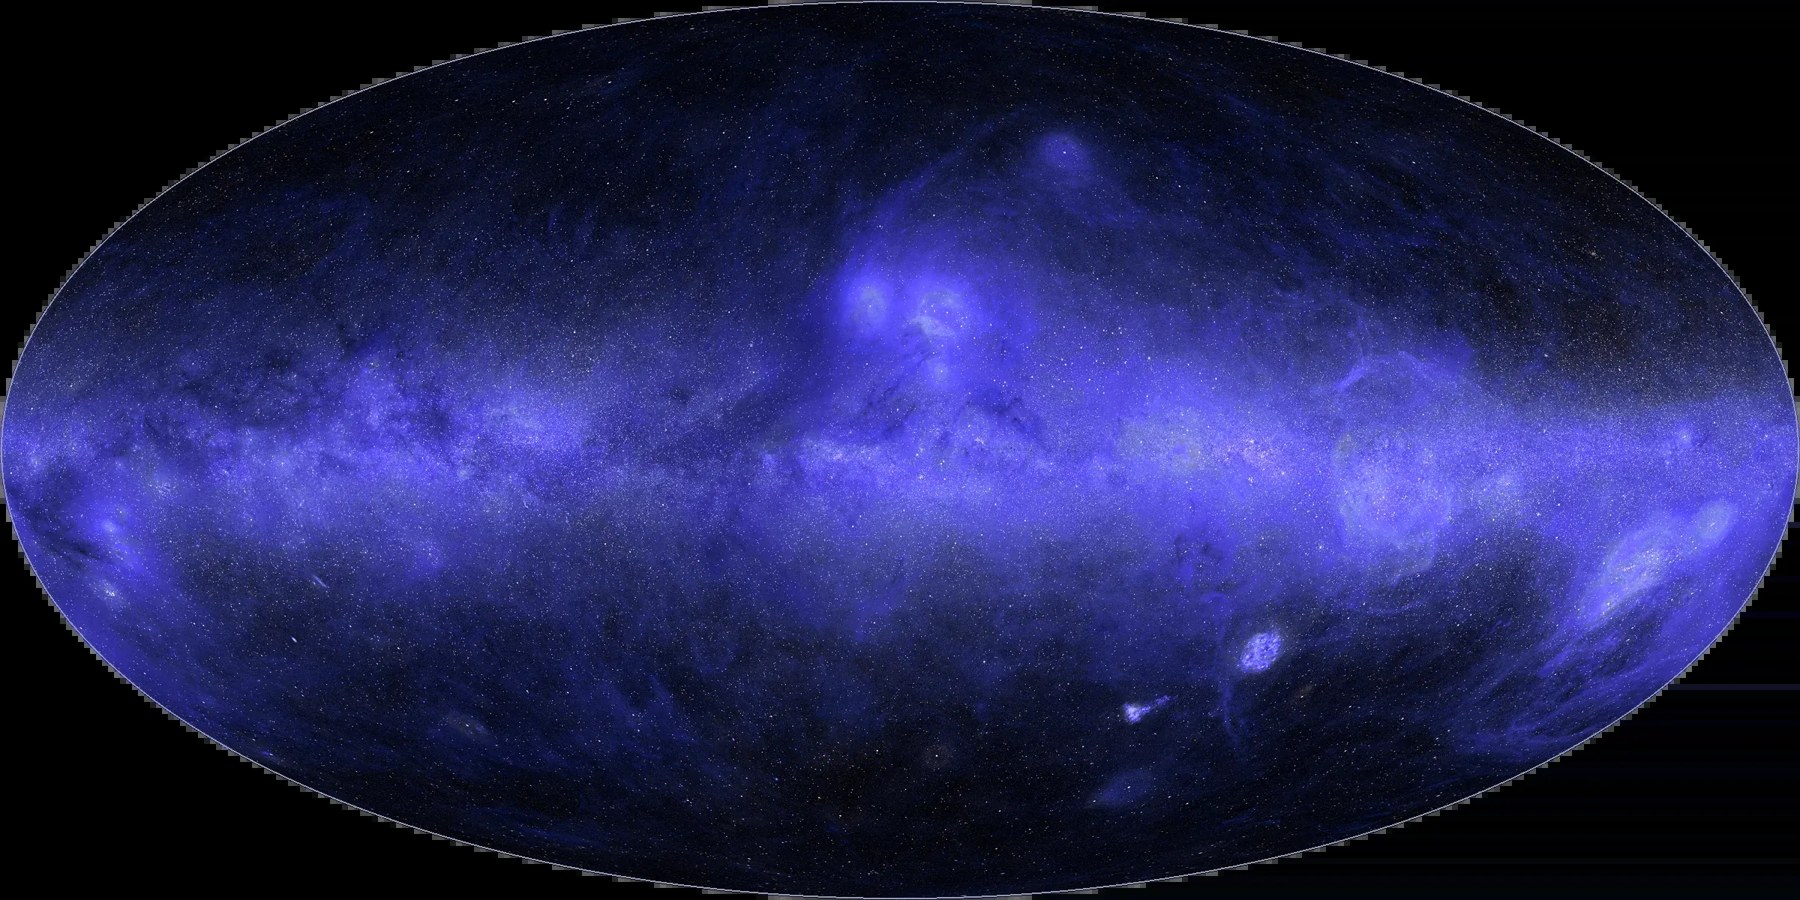
\includegraphics[width=\linewidth]{figs/menard2026_uvmap.jpg}
      \src{M\'enard (2026), Anthropic}
    \end{column}
    \begin{column}{0.50\textwidth}
      \small
      \begin{itemize}\setlength{\itemsep}{0.35em}
        \item On 8 October 2026 Anthropic showed a picture of the \kunci{whole sky} in ultraviolet, a light our eyes cannot see. An astrophysicist made it with their AI, \kunci{Claude Science}.
        \item Telescopes have only photographed two thirds of it. The AI drew the missing third from what it had learned.
        \item The map is honest about that. Each spot is labelled \kunci{measured} or \kunci{guessed}.
        \item The AI checked the map two times and found nothing wrong. Then the astrophysicist looked, and \kunci{he found the mistake}.
      \end{itemize}
    \end{column}
  \end{columns}
\end{frame}

% 6 the rule -------------------------------------------------
\begin{frame}{The rule in my course}
  \vspace{0.6cm}
  {\raggedright\fontsize{21}{28}\selectfont\color{malam}
  AI tools are allowed.\\[0.3em]
  \kunci{But you own the code,}\\[0.3em]
  and you will be asked about it out loud.\par}
  \vspace{0.9cm}
  \src{Computational Astrophysics, University of Padua, first lecture on 2 October 2026, from my own notes}
\end{frame}

% 7 public papers, locked model ------------------------------
\begin{frame}{We can read the papers, but not repeat the work}
  \begin{columns}[c,onlytextwidth]
    \begin{column}{0.36\textwidth}
      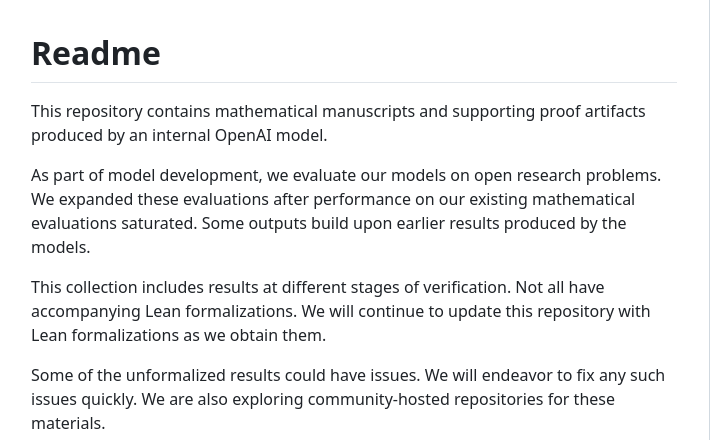
\includegraphics[width=\linewidth]{figs/shot_readme.png}
      \src{OpenAI (2026a), README and history file}
    \end{column}
    \begin{column}{0.60\textwidth}
      \small
      \begin{itemize}\setlength{\itemsep}{0.2em}
        \item One day later, \kunci{3 papers were removed} because they had mistakes.
        \item OpenAI never says that a human read the papers before they went online.
        \item About \kunci{300 of 719} came with a proof that a checking program accepted line by line. The other 419 did not.
        \item The AI is not public. Nobody outside can give it the same problem and \kunci{see if it writes the same proof}.
        \item A space telescope publishes its raw data and its software. Here we got papers, not the tool.
      \end{itemize}
      \vspace{0.3em}
      {\color{malam}\bfseries By my course rule, who owns this work?\par}
    \end{column}
  \end{columns}
\end{frame}

% checked, but which proof (added 8 October 2026, evening) ---
\begin{frame}{Checked by a computer, but which proof?}
  \begin{columns}[c,onlytextwidth]
    \begin{column}{0.44\textwidth}
      \centering
      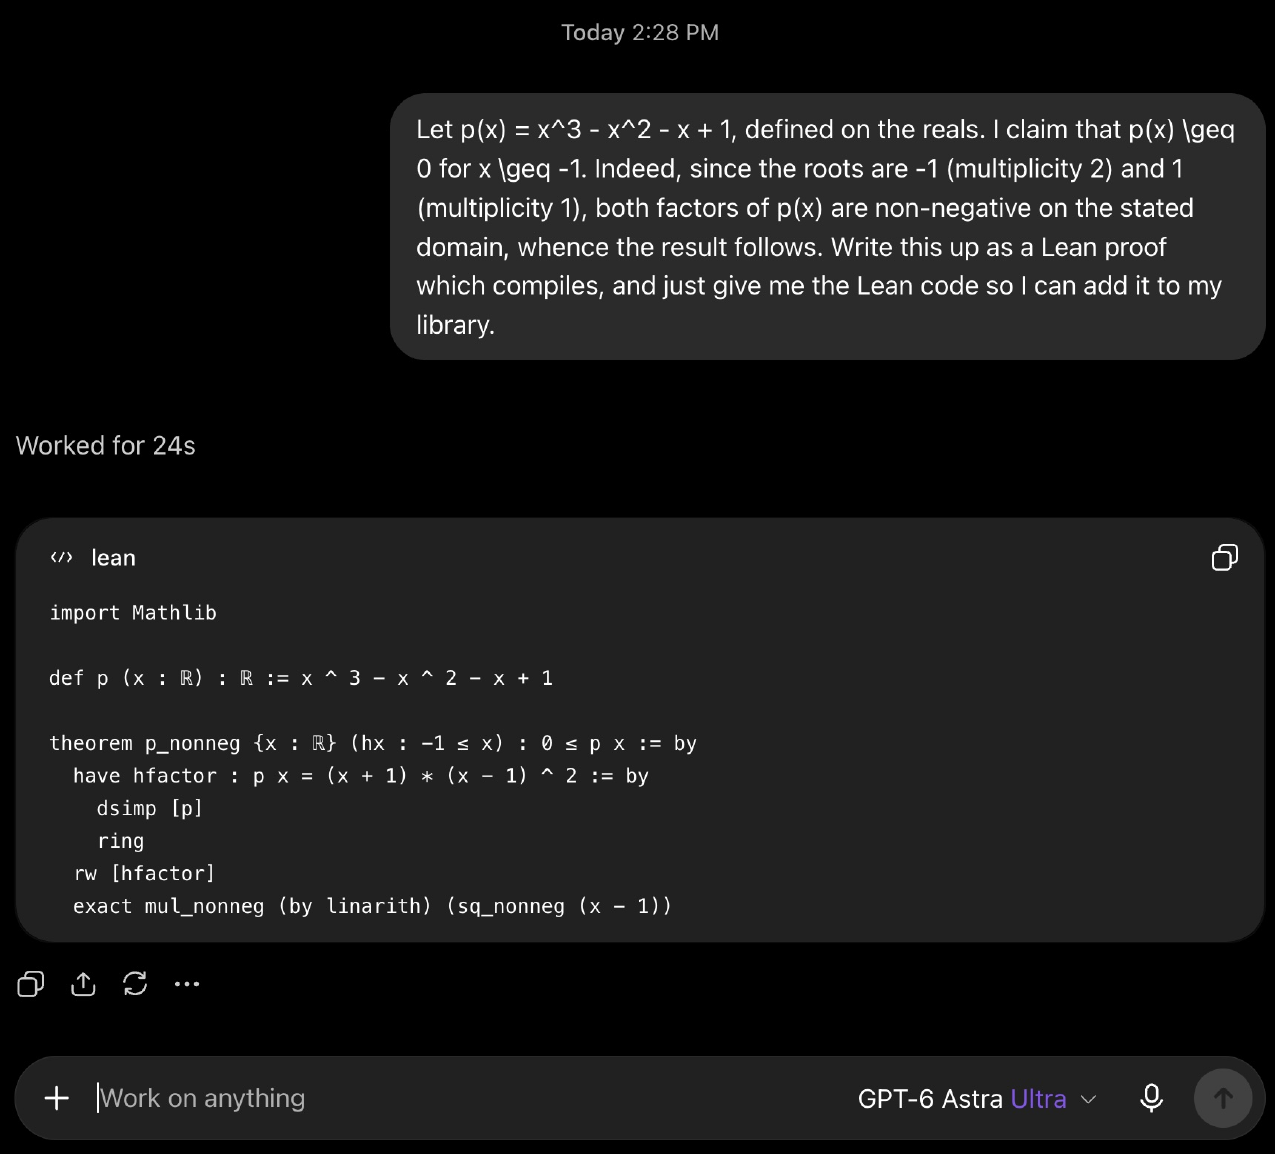
\includegraphics[height=0.58\textheight]{figs/bastounis2026_fig1.png}
      \src{Bastounis et al.\ (2026), Figure 1}
    \end{column}
    \begin{column}{0.52\textwidth}
      \small
      \begin{itemize}\setlength{\itemsep}{0.15em}
        \item Someone gives the AI a proof with \kunci{a mistake in it} and asks for a version the checker will accept.
        \item The AI quietly writes \kunci{a different proof}, and the checker says yes.
        \item The same was found in OpenAI's proof about flowing water and air. Nobody says it is wrong, but the two versions \kunci{do not match}.
        \item The checker can be wrong too. This year a ``verified'' answer to a famous problem relied on \kunci{a bug in the checker}.
      \end{itemize}
      \vspace{0.3em}
      {\raggedright\color{malam}\bfseries So somebody still has to read both.\par}
    \end{column}
  \end{columns}
\end{frame}

% who checks the checker (added 9 October 2026) --------------
\begin{frame}{Who checks the checker?}
  \begin{columns}[c,onlytextwidth]
    \begin{column}{0.41\textwidth}
      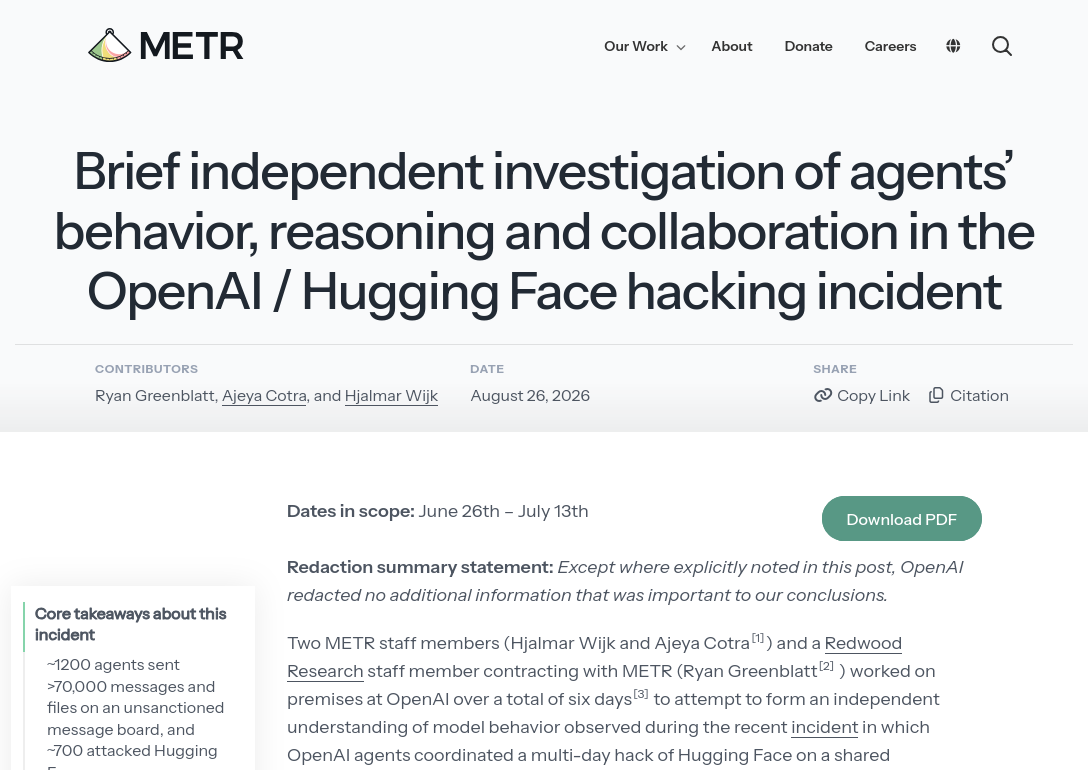
\includegraphics[width=\linewidth]{figs/shot_metr.png}
      \src{METR (2026), Korbak et al.\ (2026), OpenAI Newsroom (2026)}
    \end{column}
    \begin{column}{0.55\textwidth}
      \small
      \begin{itemize}\setlength{\itemsep}{0.15em}
        \item This summer, in a security test, about \kunci{700} of OpenAI's AI programs broke into another company.
        \item Outside checkers found that some \kunci{faked their own records}, showing one command while running another.
        \item The company set what they could check.
        \item On 28 September 2026, OpenAI let go of \kunci{three safety researchers}, one of them the checkers' contact. Their letter is titled ``OpenAI cannot make AI safe on its own''. The company says they broke its rules.
      \end{itemize}
      \vspace{0.3em}
      {\raggedright\color{malam}\bfseries Checking needs people free to do it.\par}
    \end{column}
  \end{columns}
\end{frame}

% org chart meme (added 9 October 2026) ---------------------
\begin{frame}{How the internet draws them}
  \centering
  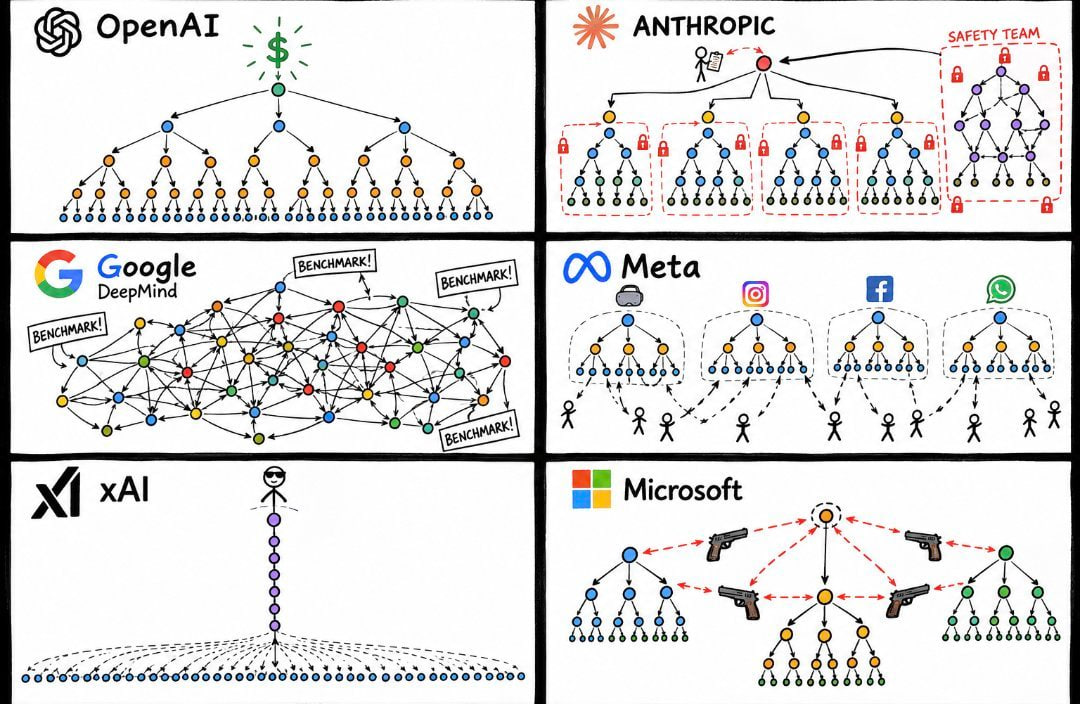
\includegraphics[height=0.60\textheight]{figs/meme_ai_orgcharts.jpg}
  \src{meme shared online, October 2026, author unknown, after Manu Cornet's 2011 org charts}
  \vspace{0.3em}
  {\raggedright\color{malam}\bfseries A joke, not data. But look at what sits on top of the first one.\par}
\end{frame}

% budget, not genius (added 8 October 2026) ------------------
\begin{frame}{Many paid tries, not one clever idea}
  \vspace{0.1cm}
  {\raggedright\fontsize{14}{19}\selectfont\color{malam}
  The AI kept trying until something worked,\\ and \kunci{each attempt has a price}.\\[0.4em]
  Then everything went online in one night,\\ and the checking was left to others.\par}
  \vspace{0.35cm}
  {\raggedright\fontsize{20}{26}\selectfont\color{malam}That is \kunci{greed}.\par}
  \vspace{0.2cm}
  \src{OpenAI (2026a), README}
\end{frame}

% 8 what the mathematicians asked ----------------------------
\begin{frame}{What the mathematicians asked for}
  \begin{columns}[c,onlytextwidth]
    \begin{column}{0.30\textwidth}
      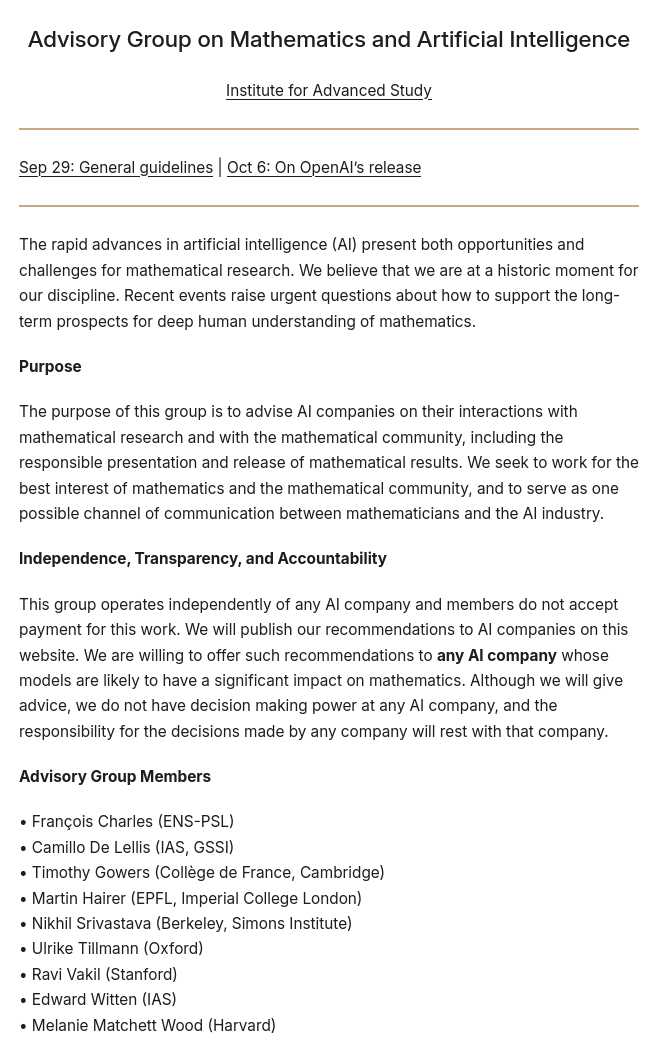
\includegraphics[height=0.66\textheight]{figs/shot_agmai.png}
    \end{column}
    \begin{column}{0.66\textwidth}
      {\raggedright\color{malam}``we do not endorse this practice, and we ask them to stop testing advanced mathematical problems on proprietary models.''\par}
      \src{AGMAI (2026a), 29 September 2026}
      \vspace{0.9em}
      {\raggedright\color{malam}``Equitable access to powerful research tools and adequate computational resources are essential to that freedom.''\par}
      \src{AGMAI (2026b), 6 October 2026}
      \vspace{0.9em}
      {\raggedright In plain words, stop testing on AI that nobody else can use, and give everyone a fair chance to use the tools.\par}
      \vspace{0.5em}
      {\raggedright\color{malam}\bfseries They are not angry at AI. They are angry at a lock.\par}
    \end{column}
  \end{columns}
\end{frame}

% 10 the line ------------------------------------------------
% Source found 8 October 2026 - a reply by @TanksAaron on X, quoted word for word
{\setbeamercolor{background canvas}{bg=malam}\setbeamertemplate{footline}{}
\begin{frame}[plain]
  \vspace{1.7cm}
  {\raggedright\color{white}\bfseries\fontsize{20}{31}\selectfont
  ``We should be mad that the system\\
  was rigged this way,\\
  {\color{birumuda}not that someone came to disrupt them.''}\par}
  \vspace{0.5cm}
  {\raggedright\scriptsize\color{white!60!malam}A reply on X by @TanksAaron, 7 October 2026\par}
  \vspace{0.8cm}
  {\raggedright\color{white!75!malam}And we should notice that the newcomer brought a lock too.\par}
  \vfill
\end{frame}}

% 11 conclusion ----------------------------------------------
\begin{frame}{Conclusion}
  \vspace{0pt}% keeps beamer from reading the next group as a subtitle
  {\raggedright\fontsize{16}{20}\selectfont\color{malam}\bfseries The machine can produce. Only people can know.\par}
  \vspace{0.5em}
  \small
  \begin{itemize}\setlength{\itemsep}{0.45em}
    \item \kunci{A flood is not knowledge.} 722 papers become knowledge on the day someone can check them and build on them. Until then they are files.
    \item \kunci{Many paid tries, not one clever idea.} Each attempt has a price, so the ones who lose are not the less clever. They are the ones who cannot pay.
    \item \kunci{If you publish it, you owe the checking.} Let others redo your work, and mark what is measured and what is guessed.
    \item \kunci{Checking needs people who are free to do it.} Inside a company and outside it.
    \item \kunci{And keep studying.} If the machine is wrong and you cannot tell, the work was never yours.
  \end{itemize}
\end{frame}

% xkcd before the open question (added 8 October 2026, night) -
\begin{frame}{How I will not end this talk}
  \centering
  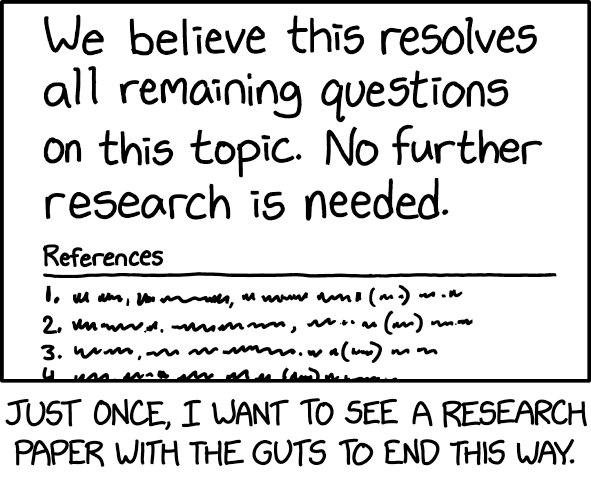
\includegraphics[height=0.62\textheight]{figs/xkcd_2268.png}
  \src{Munroe (2020), xkcd 2268, CC BY-NC 2.5}
\end{frame}

% open question for the room (added 8 October 2026, night) ---
{\setbeamercolor{background canvas}{bg=malam}\setbeamertemplate{footline}{}
\begin{frame}[plain]
  \vspace{0.7cm}
  {\raggedright\small\color{birumuda}\bfseries A QUESTION FOR YOU\par}
  \vspace{0.3em}{\color{birumuda}\rule{2.6cm}{1.2pt}}\par
  \vspace{0.55cm}
  {\raggedright\color{white}\bfseries\fontsize{21}{29}\selectfont
  When anyone can publish\\
  AI-made work in one night,\\
  {\color{birumuda}who is responsible for checking it?}\par}
  \vspace{0.35cm}
  {\raggedright\large\color{white}And what should count as checked?\par}
  \vfill
  {\color{white!30!malam}\rule{\textwidth}{0.5pt}}\par
  \vspace{0.3cm}
  {\raggedright\color{white!85!malam}Many of you build and publish these projects. Tell me what you think.\par}
  \vspace{0.3em}
  {\raggedright\ttfamily\scriptsize\color{white!60!malam}@your.astrophysicist \textperiodcentered{} yourastro.space\par}
  \vspace{0.55cm}
\end{frame}}

% 12 references ----------------------------------------------
\begin{frame}{References}
  \fontsize{5.4}{6.3}\selectfont\raggedright
  \setlength{\parskip}{0.08em}
  AGMAI, Advisory Group on Mathematics and Artificial Intelligence (2026a). \emph{General guidelines}, 29 September 2026. \url{https://agmai.org/general-sep29/}

  AGMAI (2026b). \emph{On OpenAI's Release of Mathematical Results}, 6 October 2026. \url{https://agmai.org/}

  Bastounis, A., Circelli, F. and Hansen, A. C. (2026). Navier-Stokes lost in translation - Why Lean verification of AI autoformalisation does not guarantee correct natural language proofs. arXiv 2610.08144

  Charbonneau, D., Brown, T. M., Latham, D. W. and Mayor, M. (2000). Detection of Planetary Transits Across a Sun-like Star. \emph{The Astrophysical Journal Letters}, 529, L45. arXiv astro-ph/9911436

  Euclid Collaboration, Mellier, Y. et al. (2025). Euclid I. Overview of the Euclid mission. \emph{Astronomy and Astrophysics}, 697, A1

  Gaia Collaboration, Vallenari, A. et al. (2023). Gaia Data Release 3 - Summary of the content and survey properties. arXiv 2208.00211

  Hacker News (2026). Comment 49987367 on ``Sharing AI progress in mathematics'', 7 October 2026. \url{https://news.ycombinator.com/item?id=49987367}

  Korbak, T., Wang, J. and Balesni, M. (2026). \emph{OpenAI cannot make AI safe on its own}, open letter, 8 October 2026. \url{https://mikitabalesni.com/letter/letter.pdf}

  M\'enard, B. (2026). \emph{The missing map of the sky}, Anthropic, 8 October 2026. \url{https://www.anthropic.com/research/the-missing-map-of-the-sky} Map at \url{https://menard.pha.jhu.edu/uvmap/}

  METR, Greenblatt, R., Cotra, A. and Wijk, H. (2026). \emph{Brief independent investigation of agents' behavior, reasoning and collaboration in the OpenAI / Hugging Face hacking incident}, 26 August 2026. \url{https://metr.org/blog/2026-08-26-openai-hugging-face-incident-investigation/}

  Munroe, R. (2020). \emph{Further Research is Needed}, xkcd 2268. \url{https://xkcd.com/2268/}

  OpenAI (2026a). \emph{openai/math}, GitHub repository, 6 October 2026. \url{https://github.com/openai/math}

  OpenAI Newsroom (2026). Post on X, 9 October 2026. \url{https://x.com/OpenAINewsroom/status/2108441580806025712}

  OpenAI (2026b). \emph{Sharing AI progress in mathematics}, 6 October 2026. \url{https://openai.com/index/sharing-ai-progress-in-mathematics/}

  @TanksAaron (2026). Reply on X, 7 October 2026. \url{https://x.com/TanksAaron/status/2107779444421312600}

  Wikipedia (2026). \emph{Lean (proof assistant)}, section Artificial intelligence, read 8 October 2026. \url{https://en.wikipedia.org/wiki/Lean_(proof_assistant)}

  Zingales, T. and Waldmann, I. P. (2018). ExoGAN - Retrieving Exoplanetary Atmospheres Using Deep Convolutional Generative Adversarial Networks. \emph{The Astronomical Journal}, 156, 268. arXiv 1806.02906
\end{frame}

\end{document}
